\chapter{Introducción}
\label{intro}
%\chapterquote{Hablaban siempre de dinero y planeaban asaltar un banco}{Domingo Cavallo, 2001}

Capitulo introductorio de la tesis


Algunas preguntas clave que deberian responderse en este capitulo:

¿Cuál es el campo general de estudio de tu tesis?

¿Qué fenómeno, problema o sistema estás investigando?

¿Por qué este tema es relevante científica o tecnológicamente?

¿Qué problema específico intenta resolver tu tesis?

¿Cuáles son los objetivos (generales y/o específicos)?

¿Qué enfoque metodológico utilizás? ¿Experimental, teórico, computacional?

¿Cómo está organizada la tesis?

\newpage
\section{Introducción}

Un fluido, en virtud de su masa y velocidad, puede transportar momento. Además, en virtud de su temperatura, puede transportar calor. Estrictamente hablando, la convección es el transporte de energía debido al movimiento global de un medio. Sin embargo, en ingeniería es común utilizar el término convección de forma más amplia para describir la transferencia de calor desde una superficie hacia un fluido en movimiento cuando ambos están a diferentes temperaturas \cite{cengelheat,incropera}. 

La transferencia de calor por convección puede clasificarse según la naturaleza del flujo. Hablamos de convección forzada cuando el flujo es provocado por actores externos como puede ser la acción de bombeo o un gradiente de presión; en cambio, en la convección natural, el flujo es inducido por fuerzas boyantes o de flotación, las cuales se deben a diferencias de densidad producidas por variaciones de temperatura en el propio fluido (Figura \ref{fig:natural_forzada}).

\begin{figure}[H]
 \centering
    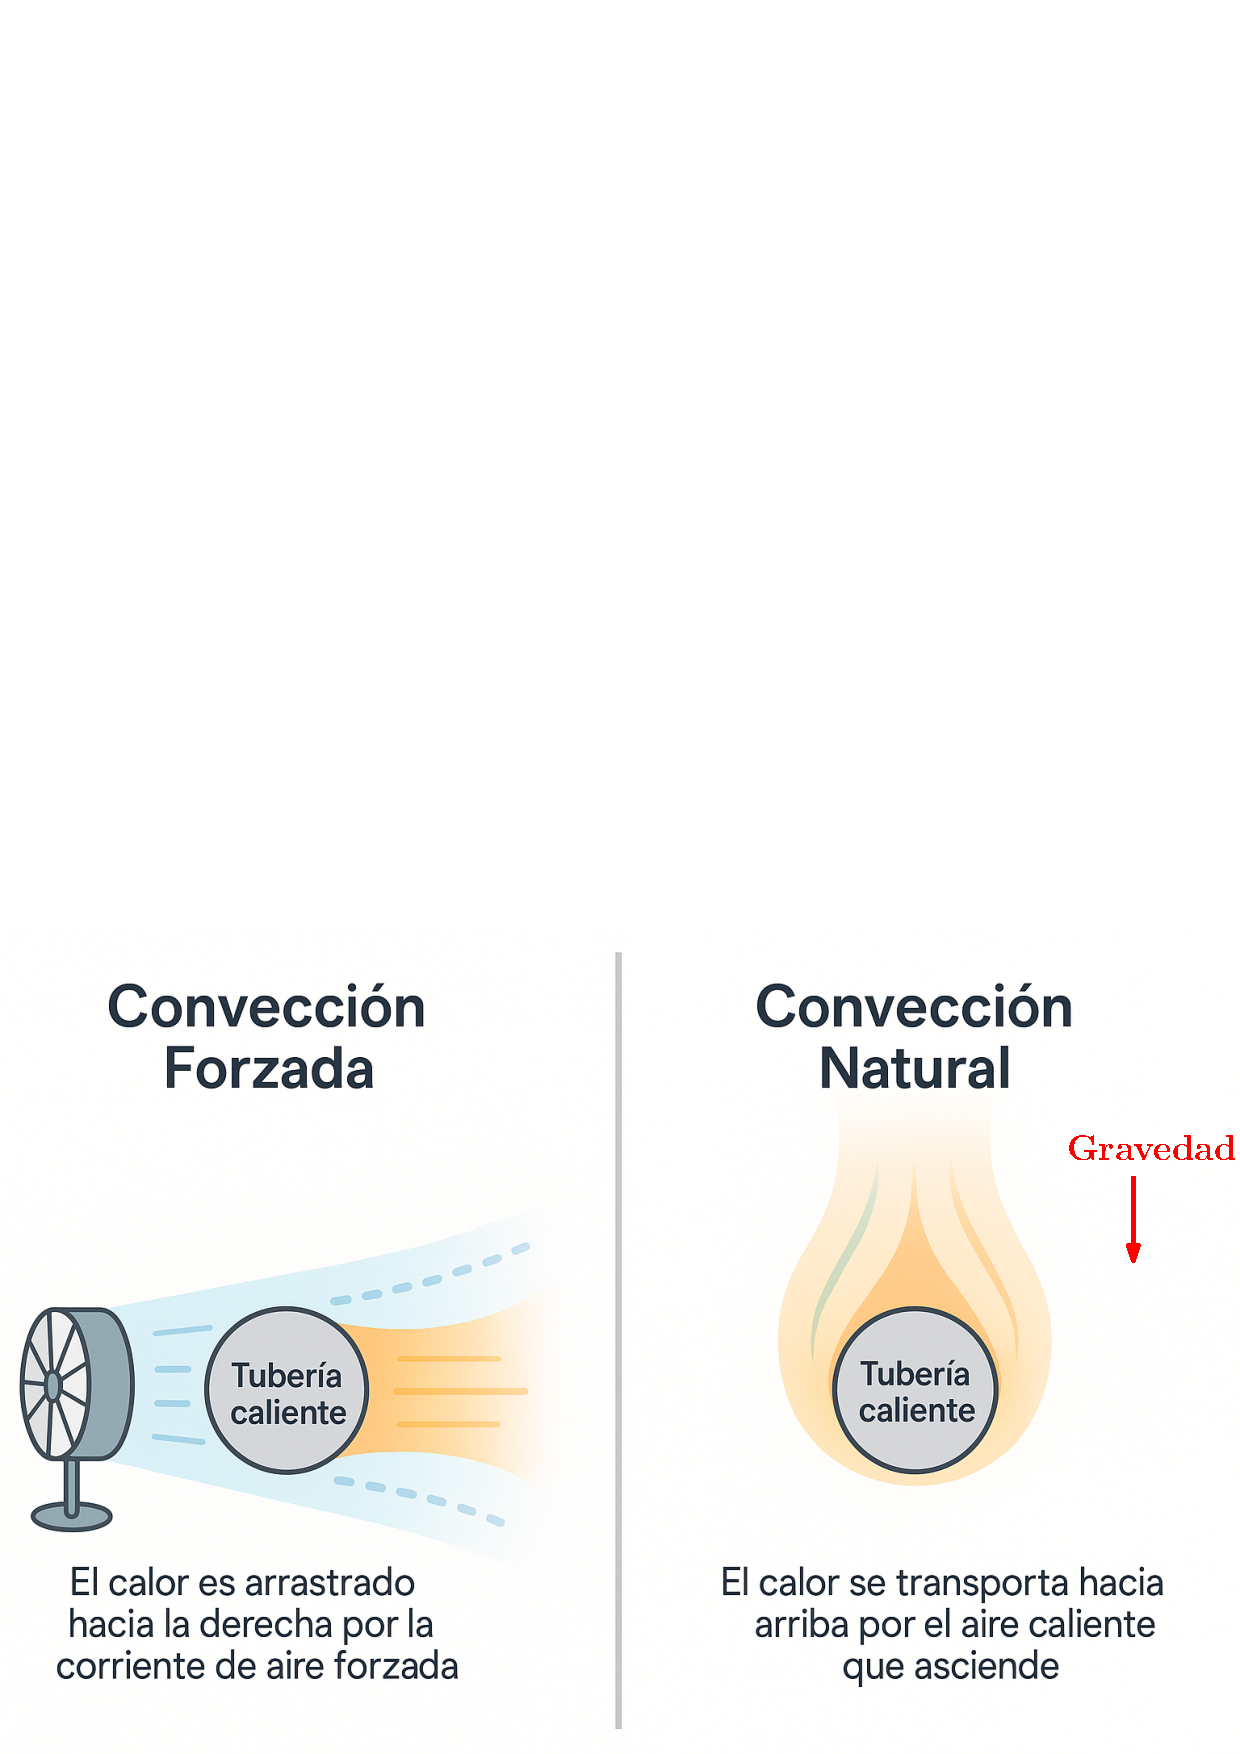
\includegraphics[width=0.6\textwidth]{figures/cap1/natural_forzada.png}
    \label{fig:natural_forzada} 
 \caption{Comparación esquemática de la transferencia de calor alrededor de una tubería caliente: (izquierda) convección forzada; (derecha) convección natural.} 
 \label{fig:natural_forzada}
\end{figure}


Los primeros estudios sobre la transferencia de calor por convección trataron las ramas de la convección forzada y la convección natural de forma separada, sin considerar la posible interacción entre ambas. Por un lado, los experimentos de Henri Bénard (1901) marcaron un hito en la comprensión de la convección natural \cite{benard1901}. Más tarde, Lord Rayleigh (1916) desarrolló la base teórica de la inestabilidad térmica en capas fluidas \cite{rayleigh1916}. En paralelo, en el ámbito de la convección forzada, trabajos como el de Dittus y Boelter (1930) establecieron correlaciones empíricas para la transferencia de calor en tubos \cite{dittus1930}. No fue sino hasta mediados del siglo XX que comenzó a reconocerse que ambos mecanismos pueden coexistir en muchas configuraciones de interés práctico. Así surgió el concepto de convección mixta, donde la convección forzada y la natural actúan simultáneamente como casos extremos de un fenómeno más general \cite{tao1960,metais1964}. 

Por otra parte, cuando un fluido se desplaza a través de un conducto o sobre una superficie, su movimiento puede clasificarse en dos tipos de régimen: laminar o turbulento. En el régimen laminar, el flujo es ordenado y las partículas del fluido se mueven en capas paralelas sin mezclarse entre sí. En cambio, en el régimen turbulento, el flujo es caótico, con remolinos, mezclas intensas y fluctuaciones en velocidad y presión. Un flujo se encuentra en un estado de transición desarrollado (esto es, no varía con el tiempo o con el espacio en un sentido de promedio estadístico), se dice que el flujo está en régimen de transición. Por otro lado, la evolución del flujo laminar a un flujo turbulento completamente desarrollado es llamada transición laminar-turbulenta. Esta transición puede ocurrir en el tiempo (transición laminar-turbulenta temporal) o en el espacio (transición laminar-turbulenta espacial).

La transición laminar-turbulenta es un fenómeno de gran importancia para la ingeniería y la física aplicada ya que puede ocurrir en diferentes dispositivos termohidráulicos. El cambio de un régimen a otro puede tener un impacto significativo en la transferencia de calor, especialmente en aplicaciones de convección mixta. El coeficiente de fricción (factor de Darcy) o el coeficiente de convección (numéro de Nusselt) se incrementan notablemente cuando se produce la transición \cite{incropera,white}. Por ejemplo, un problema importante se da en el diseño de intercambiadores de calor cuando el punto de trabajo del flujo dentro de los tubos se encuentra en régimen de transición, que es, en general, un estado intermitente en el cual parámetros tales como el coeficiente de fricción y el coeficiente de transferencia de calor tienen una gran variación \cite{ghajar2019heat}.



\textcolor{red}{Hay que poner un poco de revision bilbiografica de analisis de estabilidad lineal, capaz ... y también de revisión numerico}




\section{Motivación}


En la actualidad, muchos problemas de ingeniería presentan flujos en régimen de transición. Por citar algunos ejemplos tenemos los álabes de una turbina o los intercambiadores de calor. La mayoría de los flujos en estás condiciones son no isotérmicos \cite{chen2003direct}. 

Desde el punto de vista ingenieril, si bien éste es un régimen de trabajo no deseado por ser un estado intermitente, las características del mismo son de gran relevancia


El estudio de la transferencia de calor en la transición laminar-turbulenta es importante en diversas aplicaciones ingenieriles, como en los elementos combustibles de reactores nucleares de investigación, en intercambiadores de calor y en equipos electrónicos, entre otros. Si bien el régimen de transición no es deseado desde el punto de vista ingenieril ya que es intermitente (es decir, el flujo puede fluctuar
entre los regímenes laminar y turbulento), el estudio de la transición es relevante para poder controlar el fenómeno o anticipar, y por tanto aprovechar, su comportamiento.


La convección forzada y la convección natural son dos modos distintos de convección, que suelen combinarse y manifestarse conjuntamente en flujos ambientales y aplicaciones de ingeniería. El fenómeno de convección mixta  ocurre en procesos de fabricación de silicio, refrigeración de equipos electrónicos, paneles solares térmicos, álabes de turbinas, intercambiadores de calor de diverso tipo, reactores nucleares, entre otros \cite{kasagi1997direct}. 

Entre las aplicaciones técnicas de mayor relevancia de la convección mixta se destaca el transporte de energía térmica. En este sentido, las necesidades energéticas actuales propician el diseño y mejora constante de los reactores nucleares utilizados para la provisión de energía eléctrica. Dentro de la nueva generación de reactores nucleares GEN-IV (\url{https://www.gen-4.org/}), de los seis conceptos
especificados, uno corresponde a reactores tipo GFR (\textit{Gas-cooled Fast Reactor}) que utiliza como refrigerante gas helio cuyo numero de Prandtl es Pr$\simeq0.7$ similar al aire.





En las últimas décadas se han realizado muchos esfuerzos para desarrollar técnicas
tendientes a mejorar la transferencia de calor y el desempeño global de los intercambia-
dores de calor. El interés en estas técnicas radica en el ahorro de la energía. Con este
objetivo, se realizaron experimentos tanto en tubos como en canales, para determinar
experimentalmente las correlaciones de transferencia de calor.


Por otro lado, el estudio de la transferencia de calor en canales rectangulares ha
ganado interés en los últimos años, motivado por su aplicación en combustibles de
núcleos de reactores de investigación, en el área de sistemas electrónicos avanzados por el sistema de refrigeración



\section{Objetivos}

\section{Organización del trabajo}